\documentclass[]{article}

\usepackage{caption}
\usepackage{graphicx, subfig}
\usepackage{listings}
\usepackage[namelimits]{amsmath} 
\usepackage{fontspec}
\usepackage{amsmath}
\usepackage{amssymb}                      
\usepackage{mathrsfs}  
\usepackage{amsfonts}   
\setmainfont[Mapping=tex-text]{KaiTi}
\usepackage{fullpage}
\usepackage{amsthm}
\usepackage{fancyhdr}
\usepackage{algorithm}
\usepackage{algorithmic}
\usepackage{bm}
\usepackage{ctex}
\usepackage{txfonts}
\usepackage{tikz}
\usetikzlibrary{shapes.geometric, arrows}


%opening
\title{统计机器学习 课后作业7}
\author{陈劭涵 17300180049}



\newcommand{\tm}{\fontspec{Times New Roman}}


\begin{document}
	
\maketitle


\section{问题 (1)}
\begin{flushleft}
解:
\end{flushleft}
拉格朗日函数:\\\\
$L(w,b,\xi,\alpha,\mu)=\frac{1}{2}\vert\vert w\vert\vert^2+C\sum_{i=1}^{N}\xi_i^2-\sum_{i=1}^{N}\alpha_i[y_i(w\cdot X_i+b)-1+\xi_i]-\sum_{i=1}^{N}\mu_i\xi_i$\\\\
对偶问题:\\\\
$\mathop{max}\limits_{\alpha_i\geq0,\mu_i\geq0}\mathop{min}\limits_{w,b,\xi_i}L(w,b,\xi,\alpha,\mu)$\\\\
对$w,b,\xi_i$求导:\\\\
$\left\{\begin{matrix}
	\nabla_wL=w-\sum_{i=1}^{N}\alpha_iy_iX_i=0\\
	\nabla_bL=\sum_{i=1}^{N}\alpha_iy_i=0\\
	\nabla_{\xi_i}L=2C\xi_i-\alpha_i-\mu_i=0\\
\end{matrix}\right.$\\\\
$\therefore w=\sum_{i=1}^{N}\alpha_iy_iX_i$, $\xi_i=\frac{\alpha_i+\mu_i}{2C}$\\\\
$\therefore Q(\alpha,\mu)=\mathop{min}\limits_{w,b,\xi_i}L(w,b,\xi,\alpha,\mu)$\\\\
$=-\frac{1}{2}\sum_{i=1}^{N}\sum_{i=1}^{N}\alpha_i\alpha_jy_iy_jX_i\cdot X_j-\frac{1}{4C}\sum_{i=1}^{N}(\alpha_i+\mu_i)^2+\sum_{i=1}^{N}\alpha_i$\\\\
则对偶问题为:\\\\
$max$ $Q(\alpha,\mu)$\\
$s.t.\ \sum_{i=1}^{N}\alpha_iy_i=0$\\
$\alpha_i\geq 0$\\
$\mu_i\geq 0$\\
$i=1,2,...,N$\\\\
代入$Q(\alpha,\mu)$\\\\
可得对偶问题等价于:\\\\
$min$ $\frac{1}{2}\sum_{i=1}^{N}\sum_{i=1}^{N}\alpha_i\alpha_jy_iy_jX_i\cdot X_j+\frac{1}{4C}\sum_{i=1}^{N}(\alpha_i+\mu_i)^2-\sum_{i=1}^{N}\alpha_i$\\
$s.t.\ \sum_{i=1}^{N}\alpha_iy_i=0$\\
$\alpha_i\geq 0$\\
$\mu_i\geq 0$\\
$i=1,2,...,N$\\
\section{问题 (2)}
\begin{flushleft}
	解:
\end{flushleft}
$K(x,z)=(x\cdot z)^p$\\\\
$=(x_1z_1+x_2z_2+...+x_kz_k)^p$\\\\
$=\sum_{i_1+i_2+i_3+...+i_k=p}C_{i_1+i_2+i_3+...+i_k=p}(x_1z_1)^{i_1}(x_2z_2)^{i_2}...(x_kz_k)^{i_k}$\\\\
由于该式子中,$x_i$,$z_i$次数总是相同\\\\
定义$\phi(x)=\sqrt{C_{i_1+i_2+i_3+...+i_k=p}}x_1^{i_1}x_2^{i_2}...x_k^{i_k}$\\\\
同理$\phi(z)=\sqrt{C_{i_1+i_2+i_3+...+i_k=p}}z_1^{i_1}z_2^{i_2}...z_k^{i_k}$实际上与$\phi_(x)$相同, $\phi(z)=\phi(x)$\\\\
那么对于每种$i_1+i_2+...i_k=p$的组合,都可以定义$\phi(x)$与$\phi(z)$, 使得$C_{i_1+i_2+i_3+...+i_k=p}x_1^{i_1}x_2^{i_2}...x_k^{i_k}=\phi(x)\phi(z)$\\\\ 
我们假设有$n$种$i_1+i_2+...i_k=p$的组合, 对第$j$种组合, 定义$\phi_j(x)=\sqrt{C_j}x_1^{i_{j1}}x_2^{i_{j2}}...x_k^{i_{jk}}$\\\\
那么根据$K(x,z)$的形式,我们可以将$K(x,z)$写成$K(x,z)=\sum_{j}\phi_j(x)\phi_j(z)=\sum_{j}\phi_j(x)^2$的形式\\\\
因此内积的正整数幂是正定核函数
\section{问题 (3)}
\begin{flushleft}
	解:
\end{flushleft}
支持向量有:样本点2,3,4,6\\\\
判断原因:\\
样本点2分类正确,在间隔边界和分类边界之间, $\alpha^*_i=C,0<\xi_i<1$\\
样本点3位于错分类一侧, $\alpha^*_i=C,\xi_i>1$\\
同理样本点4也是位于错分类一侧\\
样本点6位于间隔边界上, $\alpha^*_i\leq C,\xi_i=0$\\
\section{问题 (4)}
\begin{flushleft}
	解:
\end{flushleft}
1.读入数据
\begin{lstlisting}
	data=read.csv("D:/大数据学院文件资料/2020秋课程/机器学习/assignment/homework7/simudata.csv")
	library("caTools")
	library("pROC")
	library("caret")
	library("rpart")
\end{lstlisting}
然后我阅读了文本并了解了自变量的含义,具体的自变量含义就不在这里再赘述了\\\\
2.划分数据集,用各种模型进行建模,在测试进行预测等\\\\
首先划分数据集
\begin{lstlisting}
	set.seed(1234)
	split=sample(2,nrow(data),replace=T,prob=c(0.7,0.3))
	train=data[split==1,]
	test=data[split==2,]
\end{lstlisting}
接下来我们依次用各种模型进行建模,分别是逻辑回归、kNN、决策树、Boosting 模型、随机森林、SVM,并绘制ROC曲线以及AUC值\\\\
(1) 逻辑回归模型
\begin{lstlisting}
	# logistic
	# train
	train_logis=train
	train_logis[1:26]=scale(train_logis[1:26])
	reg_log=glm(black~.,data=train_logis,family=binomial(link="logit")
	)
	summary(reg_log)
	
	# predict
	test_logis=test
	test_logis[1:26]=scale(test_logis[1:26])
	test_logis_pred=predict.glm(reg_log,newdata=test_logis,type="response")
	
	# roc and auc
	roc(test$black,as.numeric(test_logis_pred)-1,plot=TRUE,
	main="逻辑回归模型测试集ROC曲线",xlab = "FPR", ylab = "TPR",
	print.thres=TRUE,print.auc=TRUE,legacy.axes=TRUE,grid=c(0.2,0.2),
	grid.col="dimgray",auc.polygon=TRUE,max.auc.polygon=TRUE,
	auc.polygon.col="darkslategray1")
	
	test_logis_pred=test_logis_pred>0.5
	(sum(test_logis_pred==test_logis$black))/(length(test_logis_pred))
	confusionMatrix(as.factor(as.numeric(test_logis_pred)), 
	as.factor(test_logis$black))
\end{lstlisting}
具体输出结果如下:\\\\
预测准确率:
\begin{lstlisting}
	> sum(test_logis_pred==test_logis)/(length(test_logis_pred))
	[1] 0.7694257
\end{lstlisting}
可知逻辑回归模型的预测准确率为0.7694\\\\
逻辑回归模型的混淆矩阵输出为:
\begin{lstlisting}
	             Reference
	Prediction    0    1
	0            1382  351
	1             195  440
	
	Accuracy : 0.7694          
	95% CI : (0.7519, 0.7863)
	Kappa : 0.455           
	Sensitivity : 0.8763          
	Specificity : 0.5563          
	Pos Pred Value : 0.7975          
	Neg Pred Value : 0.6929          
	Prevalence : 0.6660          
	Detection Rate : 0.5836          
	Detection Prevalence : 0.7318          
	Balanced Accuracy : 0.7163          
\end{lstlisting}
逻辑回归模型的ROC曲线与AUC值为:\\\\
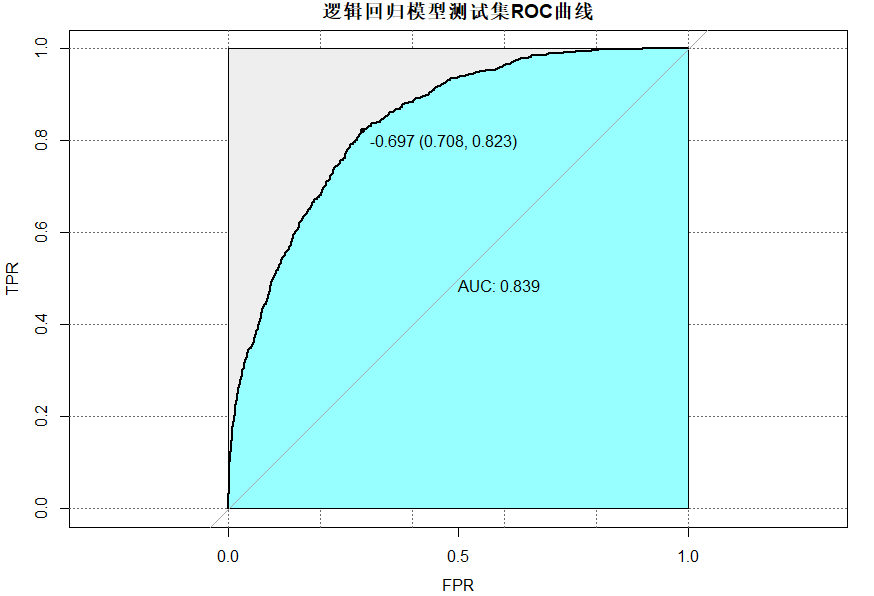
\includegraphics[width=.9\textwidth]{D:/大数据学院文件资料/2020秋课程/机器学习/homework/hw7/util/logisroc.png}\\\\\\
(2) KNN模型
\begin{lstlisting}
	# knn
	# train
	library("kknn")
	train_knn=train
	train_knn[1:26]=scale(train_knn[1:26])
	test_knn=test
	test_knn[1:26]=scale(test_knn[1:26])
	model_knn=kknn(black~.,train_knn,test_knn,k=6)
	
	# predict
	test_knn_pred=fitted(model_knn)
	test_knn_pred=test_knn_pred>0.5
	(sum(as.numeric(test_knn_pred)==test_knn$black))/(nrow(test_knn))
	confusionMatrix(as.factor(as.numeric(test_knn_pred)), 
	as.factor(test_knn$black))
	
	# roc and auc
	roc(test_knn$black,as.numeric(test_knn_pred)-1,plot=TRUE,
	main="KNN模型测试集ROC曲线",xlab = "FPR", ylab = "TPR",
	print.thres=TRUE,print.auc=TRUE,legacy.axes=TRUE,grid=c(0.2,0.2),
	grid.col="dimgray",auc.polygon=TRUE,max.auc.polygon=TRUE,
	auc.polygon.col="darkslategray1")
\end{lstlisting} 
具体输出结果如下:\\\\
预测准确率:
\begin{lstlisting}
	> (sum(as.numeric(test_knn_pred)==test_knn$black))/(nrow(test_knn))
	[1] 0.683277
\end{lstlisting}
可知KNN模型的预测准确率为0.6833\\\\
KNN模型的混淆矩阵输出为:
\begin{lstlisting}
	             Reference
	Prediction    0    1
	0            1244  417
	1            333  374
	
	Accuracy : 0.6833         
	95% CI : (0.6641, 0.702)
	Kappa : 0.2688         
	Sensitivity : 0.7888         
	Specificity : 0.4728         
	Pos Pred Value : 0.7489         
	Neg Pred Value : 0.5290         
	Prevalence : 0.6660         
	Detection Rate : 0.5253         
	Detection Prevalence : 0.7014         
	Balanced Accuracy : 0.6308              
\end{lstlisting}
KNN模型的ROC曲线与AUC值为:\\\\
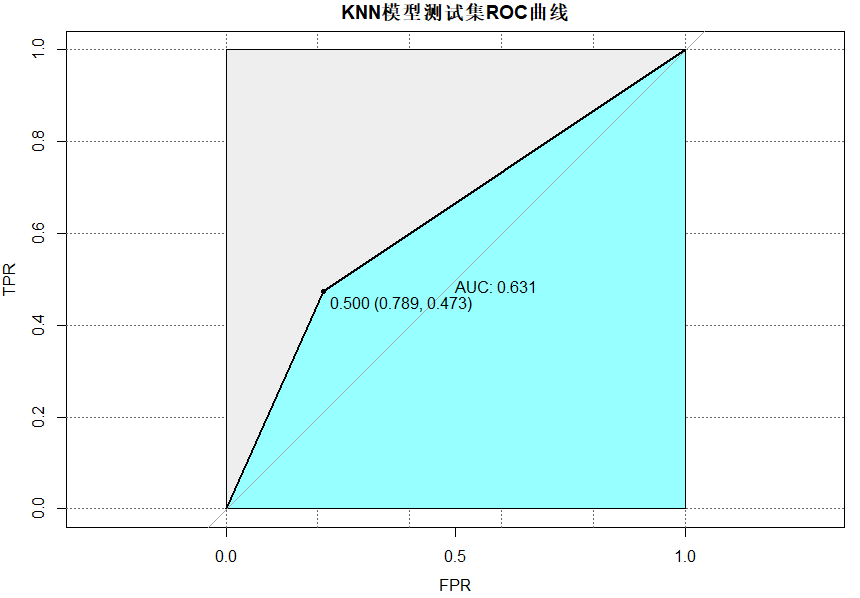
\includegraphics[width=.9\textwidth]{D:/大数据学院文件资料/2020秋课程/机器学习/homework/hw7/util/knnroc.png}\\\\\\
(3) 决策树模型
\begin{lstlisting}
	# decision tree
	# train
	train_dt=train 
	# train_dt[1:26]=scale(train_dt[1:26])  the result is better without scale
	model_dt=rpart(black~.,data=train_dt,method="class")
	
	# predict
	test_dt=test
	# test_dt[1:26]=scale(test_dt[1:26])   the result is better without scale
	test_dt_pred=predict(model_dt,test_dt,type="class")
	(sum(test_dt_pred==test_dt$black))/nrow(test_dt)
	confusionMatrix(as.factor(test_dt_pred), as.factor(test_dt$black))
	
	library(rpart.plot)
	rpart.plot(model_dt)
	
	# roc and auc
	library(rpart.plot)
	rpart.plot(model)
	
	library("pROC")
	roc(test_dt$black,as.numeric(test_pred_dt)-1,plot=TRUE,
	main="决策树测试集ROC曲线",xlab = "FPR", ylab = "TPR",
	print.thres=TRUE,print.auc=TRUE,legacy.axes=TRUE,grid=c(0.2,0.2),
	grid.col="dimgray",auc.polygon=TRUE,max.auc.polygon=TRUE,
	auc.polygon.col="darkslategray1")
\end{lstlisting} 
具体输出结果如下:\\\\
预测准确率:
\begin{lstlisting}
	> (sum(test_dt_pred==test_dt$black))/nrow(test_dt)
	[1] 0.6967905
\end{lstlisting}
可知决策树模型的预测准确率为0.6968\\\\
决策树模型的混淆矩阵输出为:
\begin{lstlisting}
	             Reference
	Prediction    0    1
	0           1426  567
	1            151  224
	
	Accuracy : 0.6968          
	95% CI : (0.6778, 0.7153)
	Kappa : 0.2157          
	Sensitivity : 0.9042          
	Specificity : 0.2832          
	Pos Pred Value : 0.7155          
	Neg Pred Value : 0.5973          
	Prevalence : 0.6660          
	Detection Rate : 0.6022          
	Detection Prevalence : 0.8416          
	Balanced Accuracy : 0.5937          
\end{lstlisting}
决策树模型的ROC曲线与AUC值为:\\\\
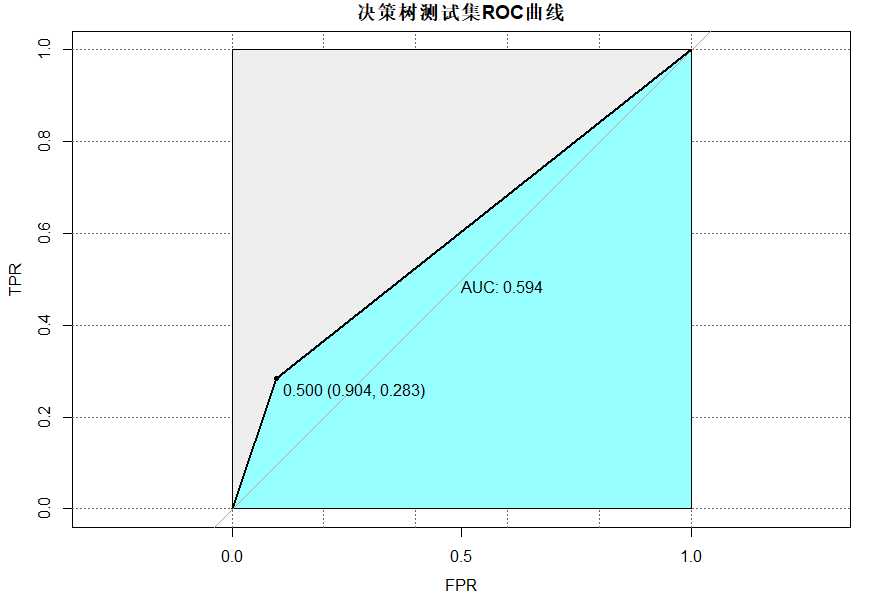
\includegraphics[width=.9\textwidth]{D:/大数据学院文件资料/2020秋课程/机器学习/homework/hw7/util/dtroc.png}\\\\\\
(5) Boosting模型
\begin{lstlisting}
	# boosting
	library("adabag")
	# train
	train_bt=train 
	train_bt[1:26]=scale(train_bt[1:26])
	train_bt$black=as.factor(train_bt$black)
	model_bt=boosting(black~.,data=train_bt)
	
	# predict
	test_bt=test
	test_bt[1:26]=scale(test_bt[1:26])  
	test_bt_pred=predict(model_bt,test_bt)
	(sum(test_bt_pred$class==test_bt$black))/nrow(test_bt)
	confusionMatrix(as.factor(as.numeric(test_bt_pred$class)), 
	as.factor(test_bt$black))
	
	# roc and auc
	roc(test_bt$black,as.numeric(test_bt_pred$class),plot=TRUE,
	main="决策树测试集ROC曲线",xlab = "FPR", ylab = "TPR",
	print.thres=TRUE,print.auc=TRUE,legacy.axes=TRUE,grid=c(0.2,0.2),
	grid.col="dimgray",auc.polygon=TRUE,max.auc.polygon=TRUE,
	auc.polygon.col="darkslategray1")
\end{lstlisting} 
具体输出结果如下:\\\\
预测准确率:
\begin{lstlisting}
	> (sum(test_bt_pred$class==test_bt$black))/nrow(test_bt)
	[1] 0.7580236
\end{lstlisting}
可知Boosting模型的预测准确率为0.7580\\\\
Boosting模型的混淆矩阵输出为:
\begin{lstlisting}
	              Reference
	Prediction    0    1
	0             1367  363
	1             210  428
	
	Accuracy : 0.758           
	95% CI : (0.7402, 0.7752)   
	Kappa : 0.4286          
	Sensitivity : 0.8668          
	Specificity : 0.5411          
	Pos Pred Value : 0.7902          
	Neg Pred Value : 0.6708          
	Prevalence : 0.6660          
	Detection Rate : 0.5773          
	Detection Prevalence : 0.7306          
	Balanced Accuracy : 0.7040            
\end{lstlisting}
Boosting模型的ROC曲线与AUC值为:\\\\
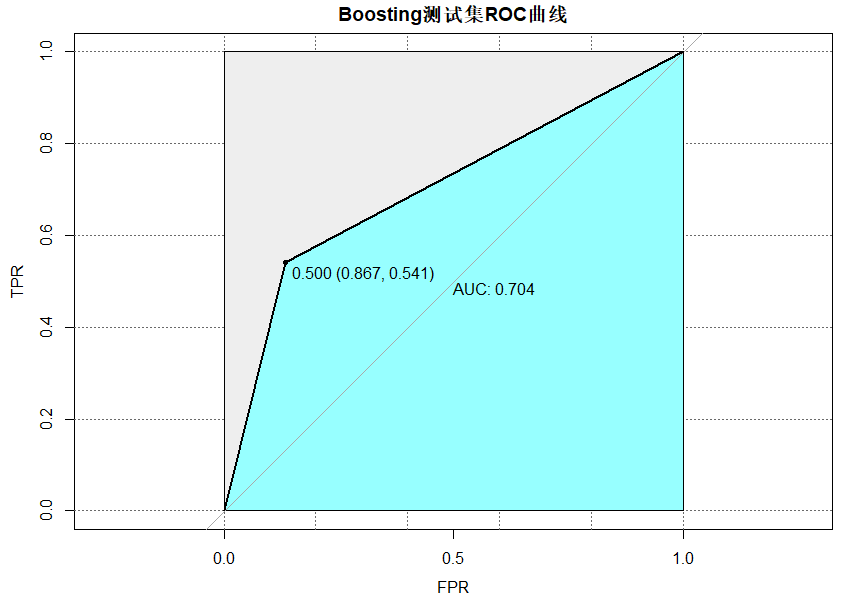
\includegraphics[width=.9\textwidth]{D:/大数据学院文件资料/2020秋课程/机器学习/homework/hw7/util/btroc.png}\\\\\\
(5) 随机森林模型
\begin{lstlisting}
	# random forest
	# train
	library("randomForest")
	train_rf=train
	train_rf[1:26]=scale(train_rf[1:26])
	model_rf=randomForest(as.factor(train_rf$black)~.,data=train_rf,importance=T)
	importance(model_rf,type=1)
	
	# predict
	test_rf=test
	test_rf[1:26]=scale(test_rf[1:26])
	test_pred_rf=predict(model_rf,test_rf)
	(sum(test_pred_rf==test_rf$black))/nrow(test_rf)
	confusionMatrix(as.factor(test_pred_rf), as.factor(test_rf$black))
	
	# roc and auc
	roc(test_rf$black,as.numeric(test_pred_rf)-1,plot=TRUE,
	main="随机森林模型测试集ROC曲线",xlab = "FPR", ylab = "TPR",
	print.thres=TRUE,print.auc=TRUE,legacy.axes=TRUE,grid=c(0.2,0.2),
	grid.col="dimgray",auc.polygon=TRUE,max.auc.polygon=TRUE,
	auc.polygon.col="darkslategray1")
\end{lstlisting} 
具体输出结果如下:\\\\
预测准确率:
\begin{lstlisting}
	> (sum(test_pred_rf==test_rf$black))/nrow(test_rf)
	[1] 0.7478885
\end{lstlisting}
可知随机森林模型的预测准确率为0.7479\\\\
随机森林模型的混淆矩阵输出为:
\begin{lstlisting}
	             Reference
	Prediction    0    1
	0            1483  503
	1            94    288
	
	Accuracy : 0.7479          
	95% CI : (0.7299, 0.7653)
	Kappa : 0.3495          
	Sensitivity : 0.9404          
	Specificity : 0.3641          
	Pos Pred Value : 0.7467          
	Neg Pred Value : 0.7539          
	Prevalence : 0.6660          
	Detection Rate : 0.6263          
	Detection Prevalence : 0.8387          
	Balanced Accuracy : 0.6522          
\end{lstlisting}
随机森林模型的ROC曲线与AUC值为:\\\\
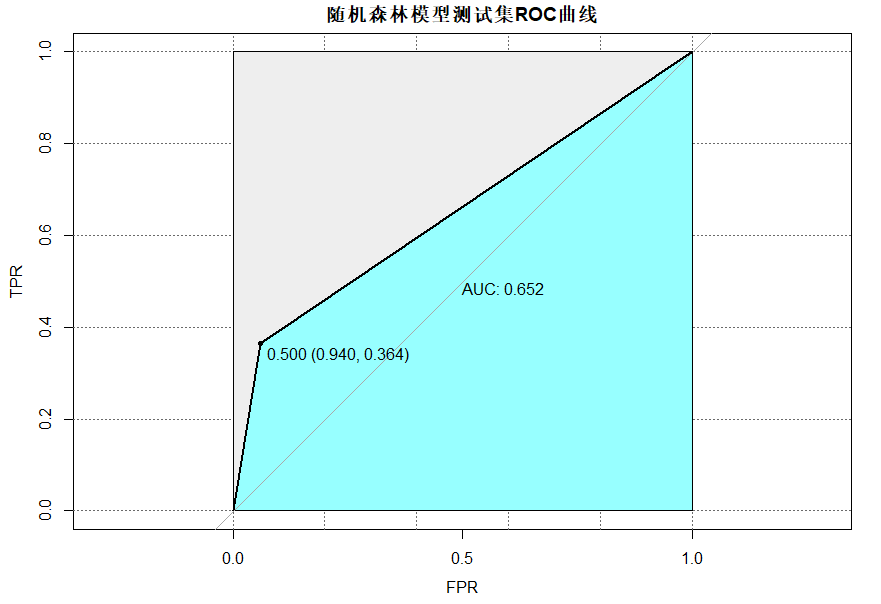
\includegraphics[width=.9\textwidth]{D:/大数据学院文件资料/2020秋课程/机器学习/homework/hw7/util/rfroc.png}\\\\\\
(6) SVM模型
\begin{lstlisting}
	# svm
	# train
	library("car")
	library("e1071")
	train_svm=train
	train_svm[1:26]=scale(train_svm[1:26])
	model_svm=svm(train_svm$black~.,data=train_svm,type="C-classification")
	
	# predict
	test_svm=test
	test_svm[1:26]=scale(test_svm[1:26])
	test_pred_svm=predict(model_svm,test_svm)
	(sum(test_pred_svm==test_svm$black))/nrow(test_svm)
	confusionMatrix(as.factor(test_pred_svm), as.factor(test_svm$black))
	
	# roc and auc
	roc(test_svm$black,as.numeric(test_pred_svm)-1,plot=TRUE,
	main="SVM模型测试集ROC曲线",xlab = "FPR", ylab = "TPR",
	print.thres=TRUE,print.auc=TRUE,legacy.axes=TRUE,grid=c(0.2,0.2),
	grid.col="dimgray",auc.polygon=TRUE,max.auc.polygon=TRUE,
	auc.polygon.col="darkslategray1")
\end{lstlisting} 
具体输出结果如下:\\\\
预测准确率:
\begin{lstlisting}
	> (sum(test_pred_svm==test_svm$black))/nrow(test_svm)
	[1] 0.7592905
\end{lstlisting}
可知SVM模型的预测准确率为0.7593\\\\
SVM模型的混淆矩阵输出为:
\begin{lstlisting}
	                Reference
	Prediction    0    1
	0            1385  378
	1            192  413
	
	Accuracy : 0.7593          
	95% CI : (0.7415, 0.7764)
	Kappa : 0.4253          
	Sensitivity : 0.8782          
	Specificity : 0.5221          
	Pos Pred Value : 0.7856          
	Neg Pred Value : 0.6826          
	Prevalence : 0.6660          
	Detection Rate : 0.5849          
	Detection Prevalence : 0.7445          
	Balanced Accuracy : 0.7002                  
\end{lstlisting}
SVM模型的ROC曲线与AUC值为:\\\\
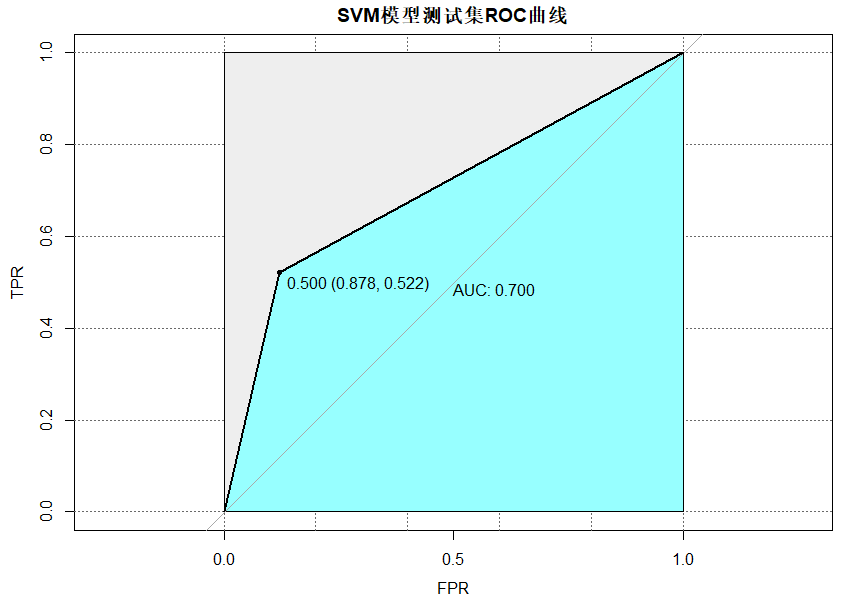
\includegraphics[width=.9\textwidth]{D:/大数据学院文件资料/2020秋课程/机器学习/homework/hw7/util/svmroc.png}\\\\\\
3.对比模型并选择最优模型\\\\
模型对比如下\\\\
ROC曲线对比:(均取p>0.5)\\
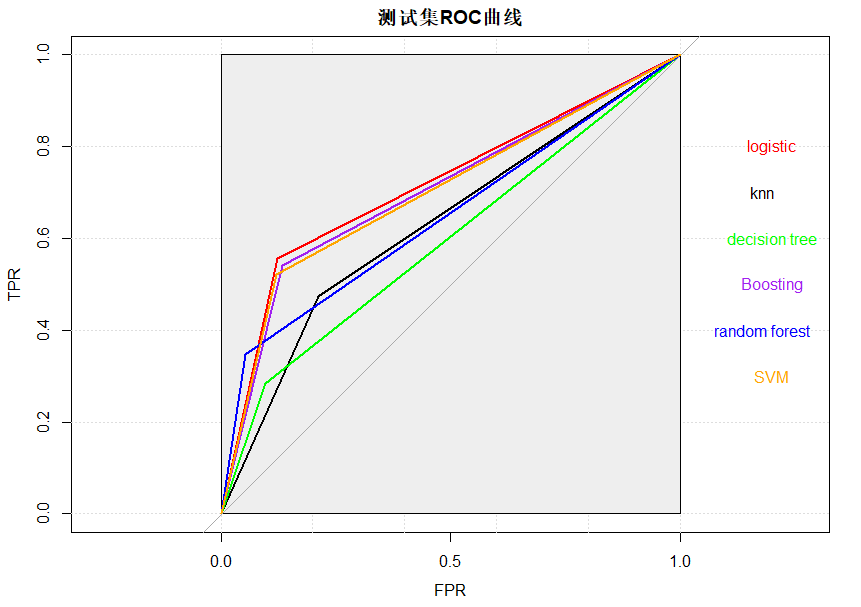
\includegraphics[width=.8\textwidth]{D:/大数据学院文件资料/2020秋课程/机器学习/homework/hw7/util/allroc.png}\\
准确度对比:(为了使对比更明显, 对准确度做了$\frac{1}{-log(accuracy)}$的操作)\\\\
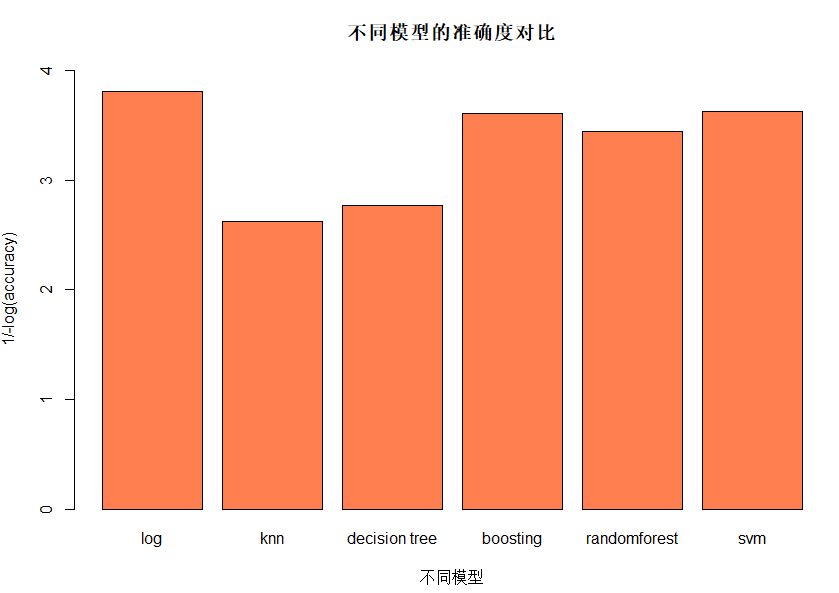
\includegraphics[width=.8\textwidth]{D:/大数据学院文件资料/2020秋课程/机器学习/homework/hw7/util/model_comparison.png}\\\\
根据ROC曲线, AUC值以及准确度对比,逻辑回归模型获得了最大的AUC值(0.839)和最高准确度(0.7694),因此选择逻辑回归模型作为最优的模型
\end{document}

